\usetikzlibrary {automata,positioning}
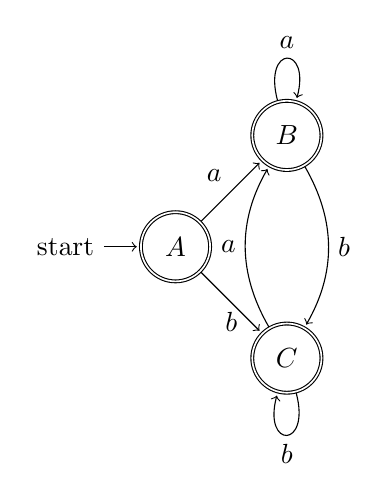
\begin{tikzpicture}[shorten >=1pt,node distance=2cm,on grid,auto]
	\node[initial,accepting,state] (A) {$A$};
	\node[accepting,state, above right of=A] (B) {$B$};
	\node[accepting,state, below right of=A] (C) {$C$};
	\path (A) edge[->] node {$a$} (B)
		(A) edge[->,below] node {$b$} (C)
		(B) edge[->,loop above] node {$a$} (B)
		(B) edge[->,bend left] node {$b$} (C)
		(C) edge[->,bend left] node {$a$} (B)
		(C) edge[->,loop below] node {$b$} (C);
\end{tikzpicture}
